\documentclass[12pt]{article}
\usepackage[tagged, highstructure]{accessibility}
\usepackage[english]{babel}
\usepackage[utf8x]{inputenc}
\usepackage[T1]{fontenc}
\usepackage[margin=1in]{geometry}
\usepackage{scribe}
\usepackage{listings}
\usepackage{natbib,verbatim}
\usepackage{amsmath,amssymb,amsfonts,mathtools}
\usepackage{bbm}
\usepackage{hyperref}
\hypersetup{
    colorlinks=true,
    linkcolor=blue,
    filecolor=magenta,      
    urlcolor=magenta,
    citecolor=magenta,
    pdftitle={Homework 4},
    pdfauthor={Nisha Chandramoorthy},
    pdflang={en-US}
}

%\Scribe{Your Name}
\title{Homework 4_6740}
\LectureNumber{CSE 6740}
\LectureDate{Due Dec 1st, '23 (11:59 pm ET) on Gradescope} 
\Lecturer{Cite any sources and collaborators; do not copy. See syllabus for policy.}
\LectureTitle{Homework 4: Unsupervised learning}

\lstset{style=mystyle}

\begin{document}
\MakeScribeTop
%----------------------------------------------------------------------------------
\section{Maximum Likelihood [15 pts]}

Suppose we have $m$ i.i.d. samples from the following probability distribution. This
problem asks you to build a log-likelihood function, and find the
maximum likelihood estimator of the parameter(s).

\subsection*{(a) Multinomial distribution [5 pts]}
The probability density function of Multinomial distribution is given by 
$$f(x_1,x_2,\dots,x_k;n,\theta_1,\theta_2,\dots,\theta_k)=\frac{n!}{x_1!x_2!\cdots x_k!}\prod_{j=1}^{k}\theta_j^{x_j},$$
where $\sum_{j=1}^k\theta_j=1,\sum_{j=1}^k x_j=n$. What is the maximum likelihood estimator of $\theta_j, j=1,\dots k$?

\subsection*{(b) Gaussian normal distribution [5 pts]}
Suppose we have $m$ i.i.d. samples from a multivariate Gaussian normal distribution on $\mathbb{R}^d,$ 
$\mathcal{N}(\mu, \Sigma)$, which is given by
\begin{equation}
	\mathcal{N}(x; \mu, \Sigma) = \frac{1}{|\Sigma|^{1/2} \sqrt{2\pi}^d} \exp
	\left( - (x - \mu)^\top \Sigma^{-1} (x - \mu)\right).\nonumber
\end{equation}
What is the maximum likelihood estimator of $\mu$ and $\Sigma$? (4 points) Is the ML estimator of $\Sigma$ biased? (1 point)
\vspace{1cm}

\subsection*{(c) Exponential distribution [5 pts]}
The probability density function of Exponential distribution is
given by
\begin{equation} \nonumber
f(x) = \left\{\begin{matrix}
\lambda e^{-\lambda x} & x \ge 0\\
0 & x < 0
\end{matrix}\right.
\end{equation}
What is the maximum likelihood estimator of $\lambda$?

%----------------------------------------------------------------------------------
\section{$k$-means clustering [15 pts]}

Given $m$ data points $\text x_i (i=1,\dots,m)$, $k$-means clustering algorithm groups them into $k$ clusters by minimizing the distortion function over $\{ r^{ij}, \mu^j \}$
$$J=\sum_{i=1}^m\sum_{j=1}^kr^{ij} \|\text x_i-\mu^j\|^2,$$
where $r^{ij}=1$ if $\text x_i$ belongs to the $j$-th cluster and $r^{ij}=0$ otherwise.

\subsection*{ Part (a)}
Prove that using the squared Euclidean distance $\|\text x_i-\mu^j\|^2$ as the dissimilarity function and minimizing the distortion function, we will have 
   $$\mu^j=\frac{\sum_i r^{ij} \text x_i}{\sum_i r^{ij}}.$$
   That is, $\mu^j$ is the center of $j$-th cluster. [5 pts]

\subsection*{ Part (b)}
Suppose at each iteration, we need to find two clusters $\{\text x_1, \text x_2, \dots, \text x_p\}$ and $\{\text y_1, \text y_2, \dots, \text y_q\}$ with the minimum distance to merge. Some of the most commonly used distance metrics between two clusters are:
    \begin{itemize}
    \item Single linkage: the minimum distance between any pairs of points from the two clusters, i.e.
    $$\min_{i=1,\dots,p \atop j=1,\dots, q}\|\text x_i - \text y_j\|$$
    \item Complete linkage: the maximum distance between any parts of points from the two clusters, i.e.
    $$\max_{i=1,\dots,p \atop j=1,\dots, q}\|\text x_i - \text y_j\|$$
    \item Average linkage: the average distance between all pair of points from the two clusters, i.e.
    $$\frac{1}{mp}\sum_{i=1}^p\sum_{j=1}^q\|\text x_i - \text y_j\|$$
    \end{itemize}

Which of the three cluster distance metrics described above would most likely result in clusters most similar to those given by $k$-means? (Suppose $k$ is a power of 2 in this case). [5 pts]

\subsection*{Part c}
For the \emph{two moons} data (Figure \ref{fig:twomoons}), which of these three distance metrics (if any) would successfully separate the two moons? [5 pts]
\begin{figure}[h]
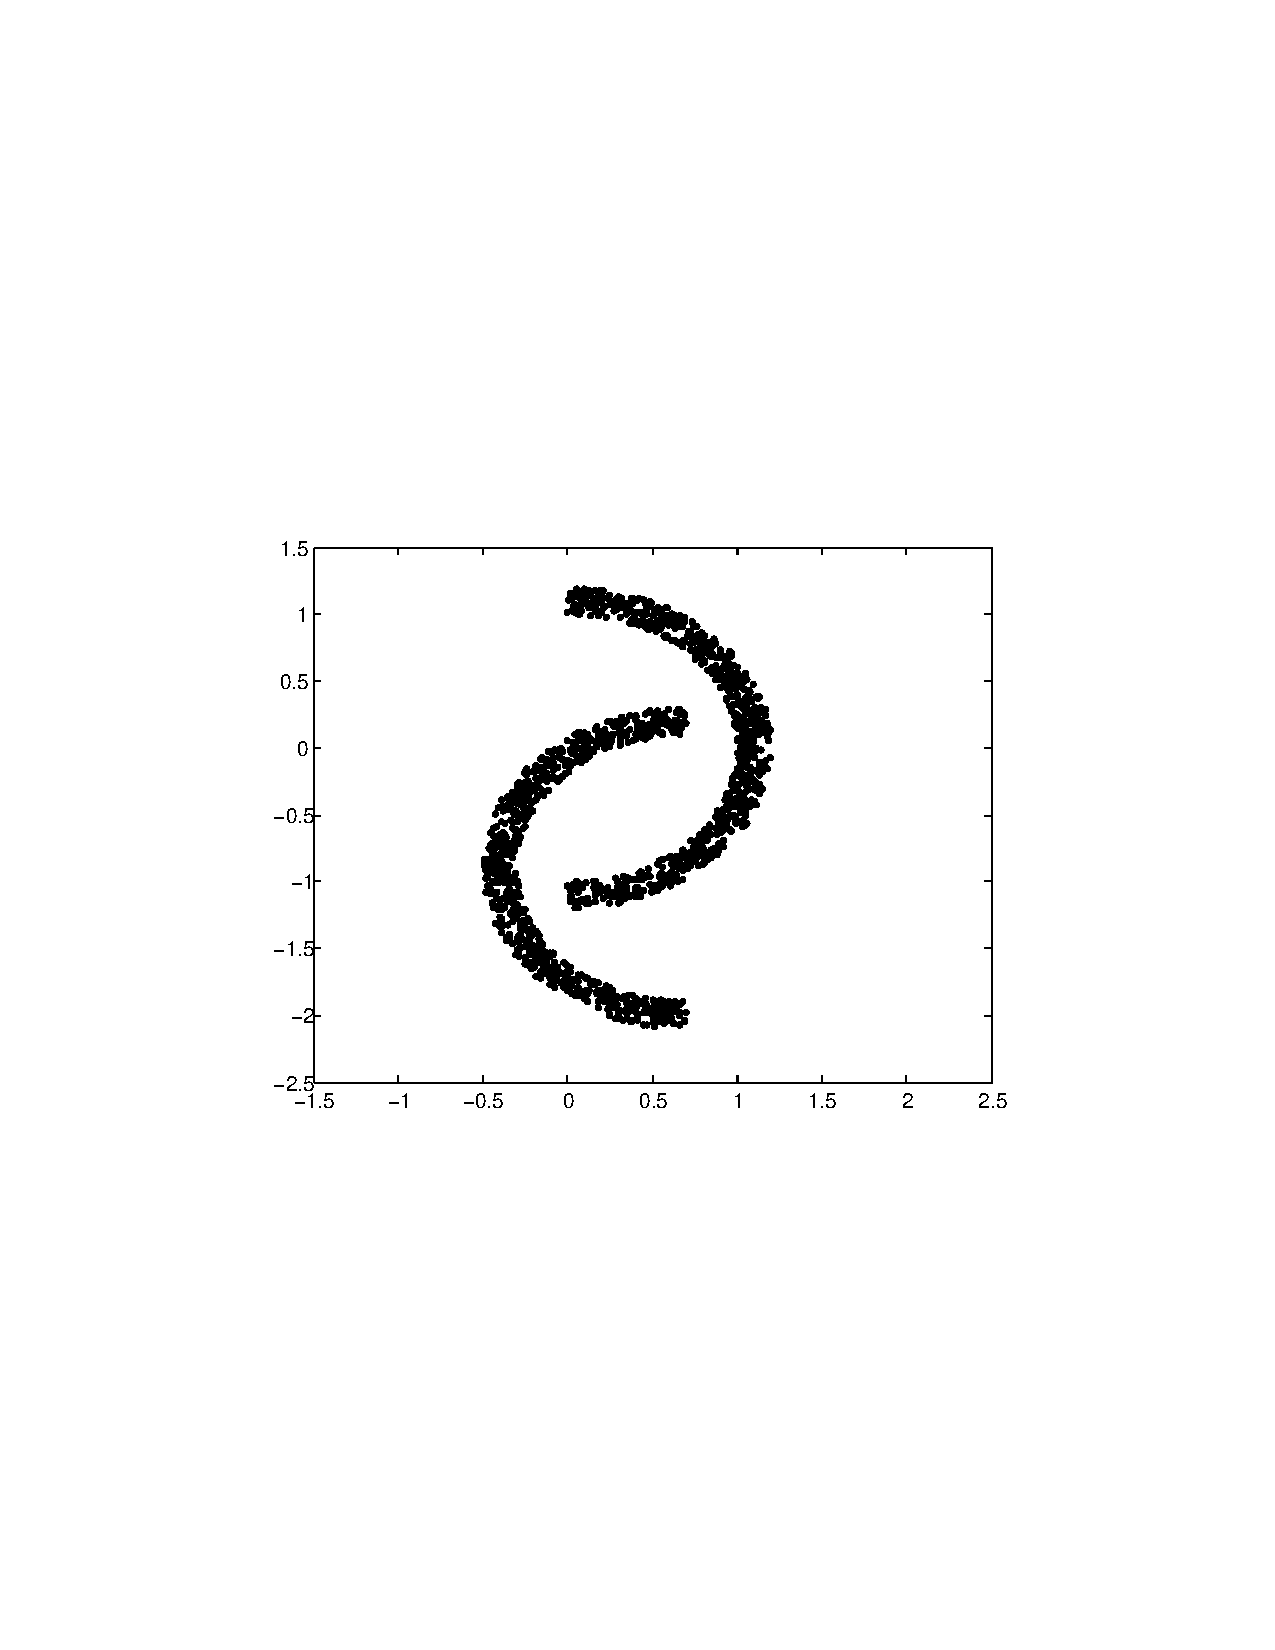
\includegraphics[trim = 0mm 90mm 0mm 90mm, clip, width = \linewidth]{clustering}
\caption{Two moons data}
	\label{fig:twomoons}
\end{figure}
\vspace{1cm}




\bibliographystyle{plain}
\bibliography{refs}
\end{document}
